\documentclass{beamer}
\usetheme{default}

\usepackage{graphicx}
\DeclareMathOperator*{\argmax}{arg\,max}
\DeclareMathOperator*{\argmin}{arg\,min}
\DeclareMathOperator*{\Var}{Var}
\DeclareMathOperator*{\COV}{Cov}

\newcommand{\expSym}{{E}}
\newcommand{\E}[1]{\ensuremath{\expSym\left(#1\right)}}
\newcommand{\prob}[1]{\ensuremath{\Pr\left(#1\right)}}
\newcommand{\T}{T}
\newcommand{\Cov}[2]{\ensuremath{\COV(#1, #2)}}

\renewcommand{\vec}[1]{\ensuremath{#1}}

\usepackage{amsmath}
\usepackage{amssymb}
\usepackage{amsthm}
\usepackage{multirow}
\usepackage{mathtools}

\setbeamertemplate{footline}[frame number]

\title{Analysis of Markovian Population Models}
\subtitle{Dissertation Defense}
\author{Michael Backenk\"{o}hler}
\institute{Saarland Informatics Campus}
\date{September 20, 2022}

\begin{document}

\begin{frame}
\titlepage
\end{frame}

\begin{frame}{Motivation}
  \begin{itemize}
    \item Example
    \item list other applications: queueing, metabolic networks, switches etc.
  \end{itemize}
\end{frame}

\begin{frame}{Markovian Population Models}{Semantics}
  \begin{itemize}
    \item counting agents / population size
    \item continuous time
    \item exponential jump times / CTMC dynamics
  \end{itemize}
\end{frame}

\section{Markovian Population Models}
\begin{frame}{Markovian Population Models}{Stationary Distribution -- Foster-Lyapunov Functions}
    \begin{itemize}
        \item ergodic chains converge to unique distribution
        \item how does this distribution look like for infinite state-spaces?
        \item use Foster-Lyapunov function to bound sets
        \item locally augment functions for tighter sets / bounds
    \end{itemize}
\end{frame}

\begin{frame}{Markovian Population Models}{Moment Dynamics}
  \begin{itemize}
    \item alternative approach: look at moments instead of states
    \item expected values, e.g. $\E{X}, \E{X^2}$
    \begin{figure}
        \centering
    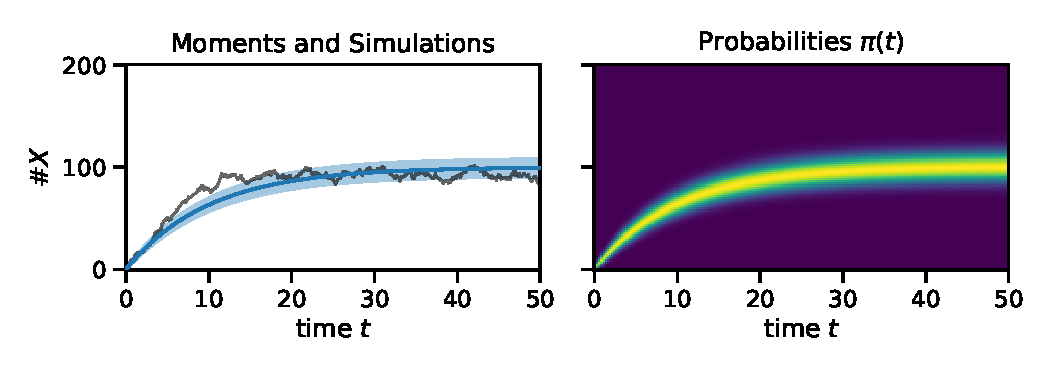
\includegraphics[scale=.4]{../gfx/momsandprobs.pdf}
    \end{figure}
    \item Moment formula
        \begin{equation*}
            \frac{d}{dt}\E{f({\vec{ X}}_t)} = \sum_{j=1}^{n_R}\E{\left(f({\vec X_t +
            \vec{v}_j}) - f(\vec X_t)\right)\alpha_j(\vec X_t)}
        \end{equation*}
    \item ODE system not closed
  \end{itemize}
\end{frame}

\begin{frame}{Markovian Population Models}{Martingale Process}
    \begin{itemize}
    \item Analytic integration and resulting martingale process
        \begin{equation*}
            \begin{split}
            Z_T\coloneqq&\,w(T)f(\vec X_T) - w(0)f(\vec X_{0}) -
            \int_{0}^T\frac{dw(t)}{dt}f(\vec X_t)\,dt\\
            &-\sum_{j=1}^{n_R}\int_{0}^Tw(t)
                 (f(\vec X_t+\vec v_j) - f(\vec X_t))\alpha_j(\vec X_t)\,dt\,.
         \end{split}
        \end{equation*}
    \item Crucially, $\E{Z_T}=0$, $\forall T\geq 0$.
  \end{itemize}
\end{frame}

\section{Bounding Mean First-Passage Times}
\begin{frame}{Bounding Mean First-Passage Times}{Martingale Process and Linear Moment Constraints}
  \begin{itemize}
      \item expected occupation time and exit measures (in relation to expectation of the martingale)
      \item linear constraints connecting 3 measures (integrate moms and figure)
  \end{itemize}
    \begin{figure}
        \centering
        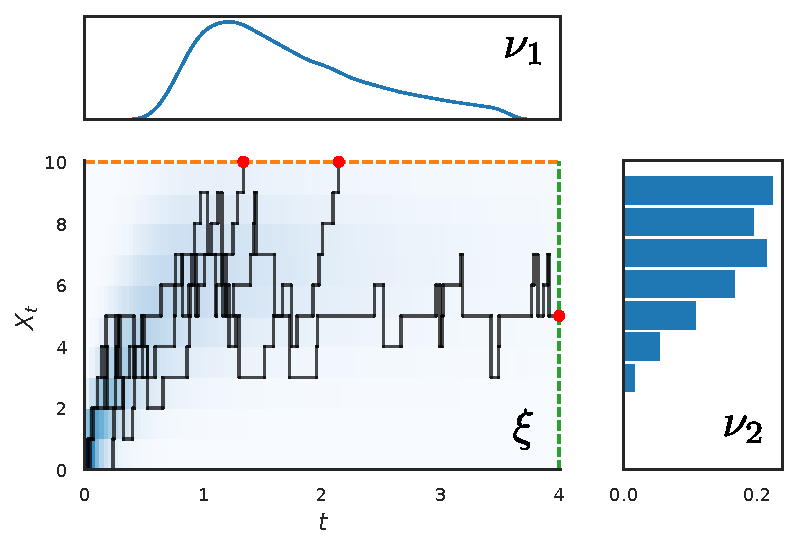
\includegraphics[scale=.4]{../gfx/decomp1.pdf}
    \end{figure}
\end{frame}

\begin{frame}{Bounding Mean First-Passage Times}{Moment Matrices and Semi-Definite Programs}
  \begin{itemize}
    \item semi-definite moment constraints (positive variance as example)
    \item hint at localizing matrices
  \end{itemize}
\end{frame}

\begin{frame}{Bounding Mean First-Passage Times}{Results and Practical Issues}
  \begin{itemize}
    \item moment stiffness, re-scaling issue
    \item some examples
  \end{itemize}
\end{frame}

\begin{frame}{Bounding Mean First-Passage Times}{Hausdorff Constraints and Linear Programs}
  \begin{itemize}
    \item linear constraints possible if domains (time and space) are finite
    \item 1D visualization of Hausdorff constraints
  \end{itemize}
\end{frame}

\section{Linear Control Variates}
\begin{frame}{Linear Control Variates}{Using Correlated RVs with Known Expected Value}
  \begin{itemize}
    \item segue: use the same martingale constraints to enhance MC estimation
    \item use correlations between target RV and martingales (linear regression, i.e.\ control variates)
  \end{itemize}
\end{frame}

\begin{frame}{Linear Control Variates}{Finding Efficient Sets of Control Variates}
  \begin{itemize}
    \item time-weighting has a large influence on the correlation
    \item Infinitely many possibilities (cost needs to be controlled though)
    \item variates can be highly redundant (correlated) and incur an additional cost
    \item Alg.~1: Tighten an initial proposal set
    \item Alg.~2: Re-sample promising candidates
  \end{itemize}
\end{frame}

\begin{frame}{Linear Control Variates}{Results}
  \begin{itemize}
    \item best example?
  \end{itemize}
\end{frame}

\section{State-Space Aggregation}
\begin{frame}{State-Space Aggregation}{Treating Hyper-Cubes of States as One}
    \begin{columns}
        \begin{column}{.4\textwidth}
            \begin{figure}
            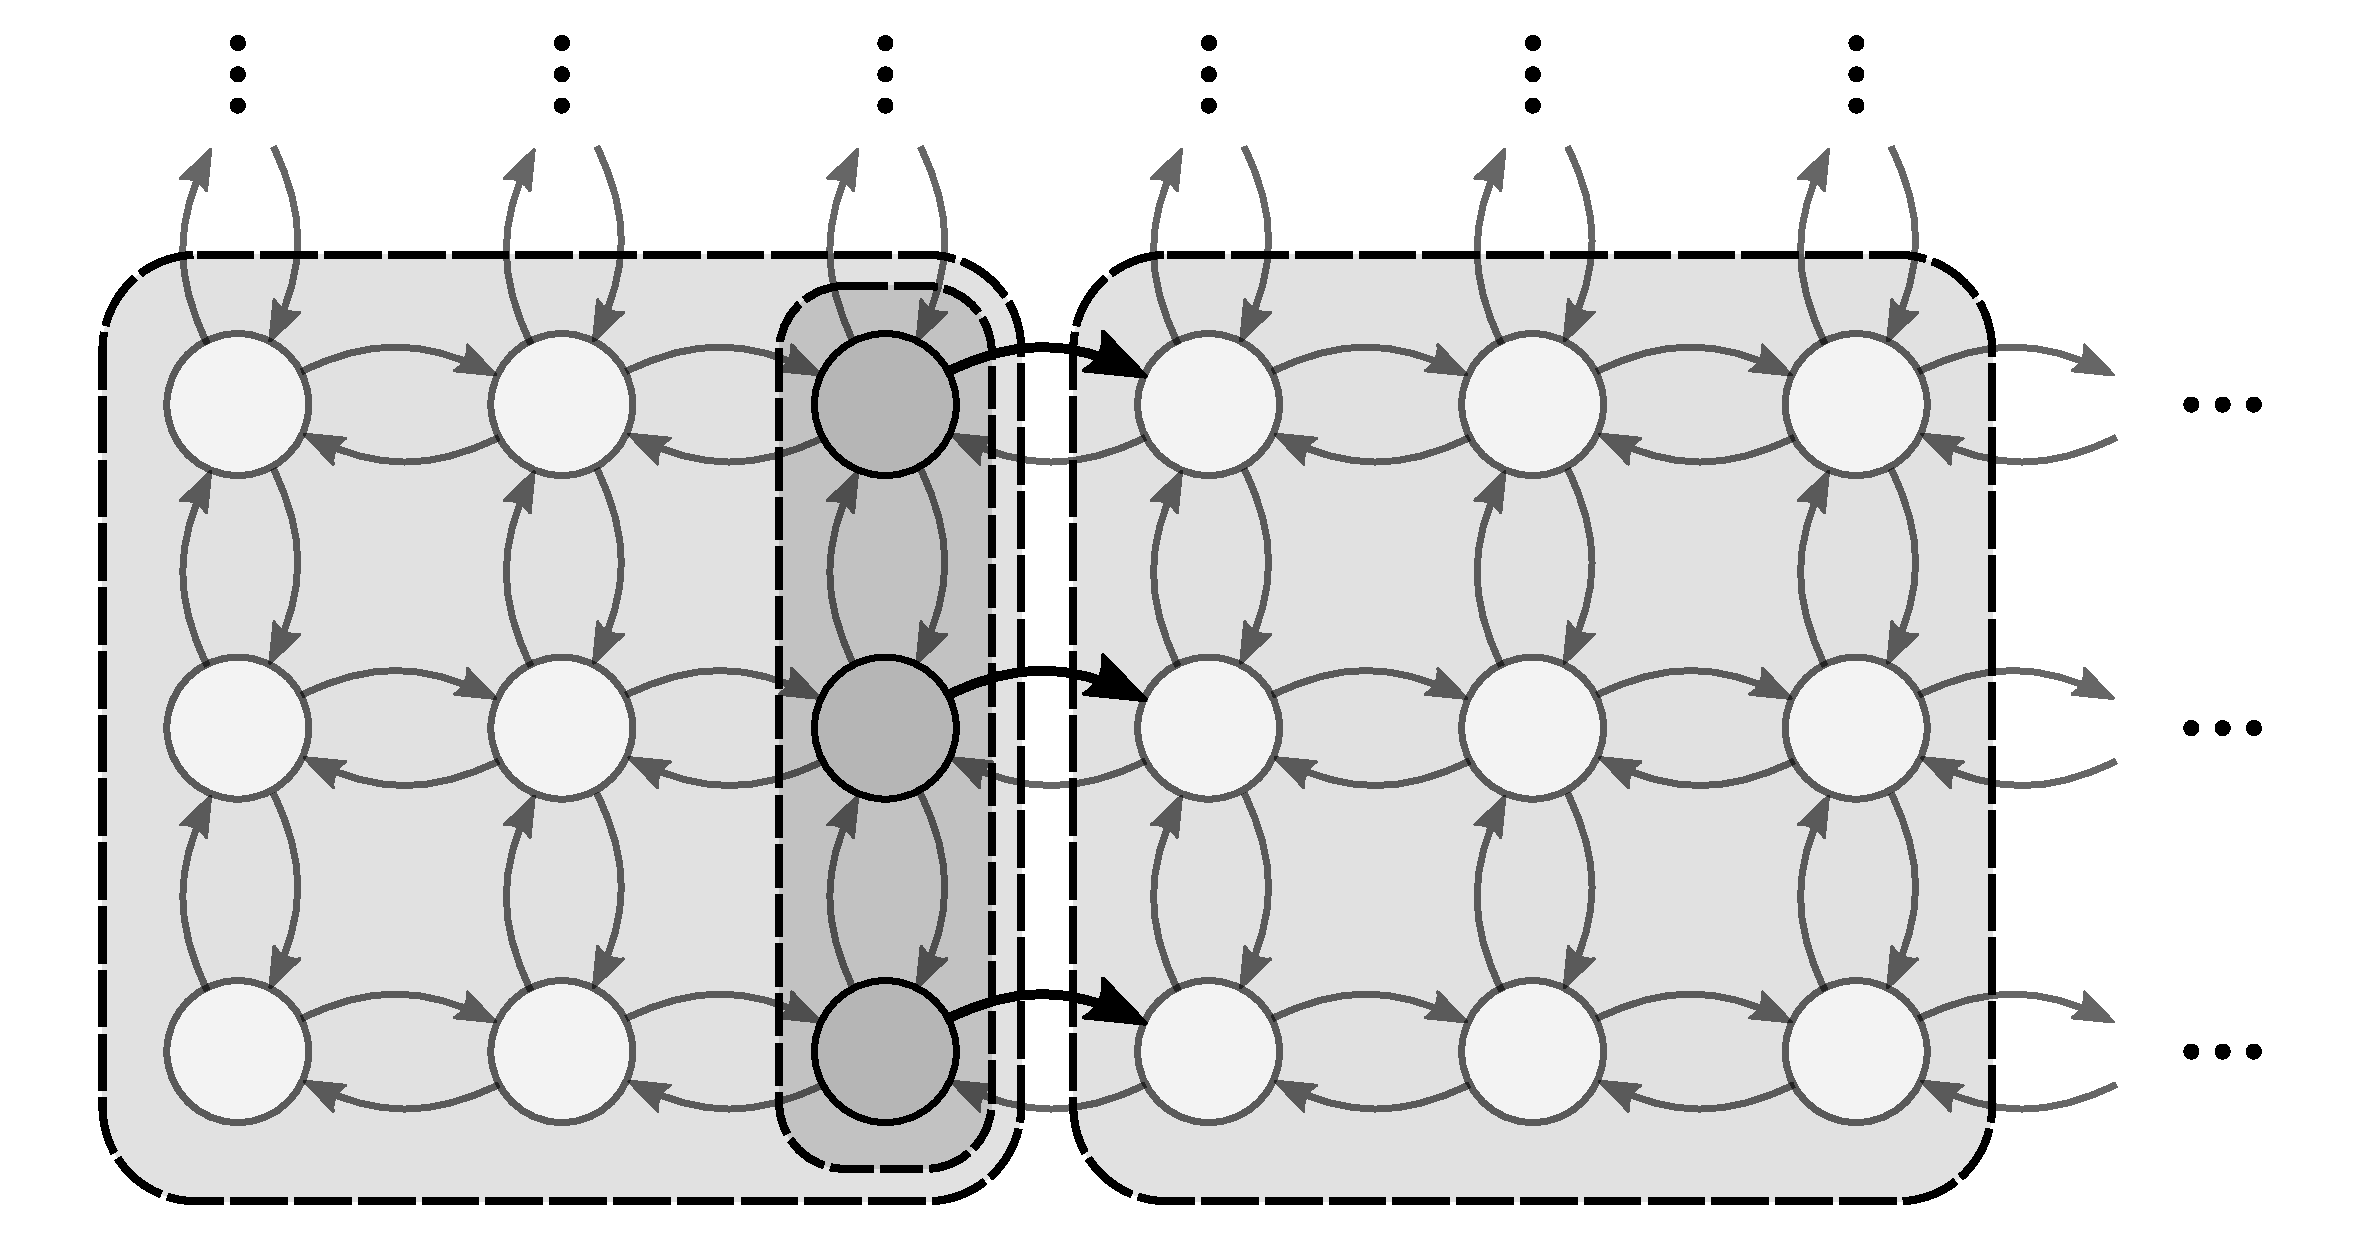
\includegraphics[width=5cm]{../gfx/macro_states.pdf}
            \end{figure}
            \begin{figure}
                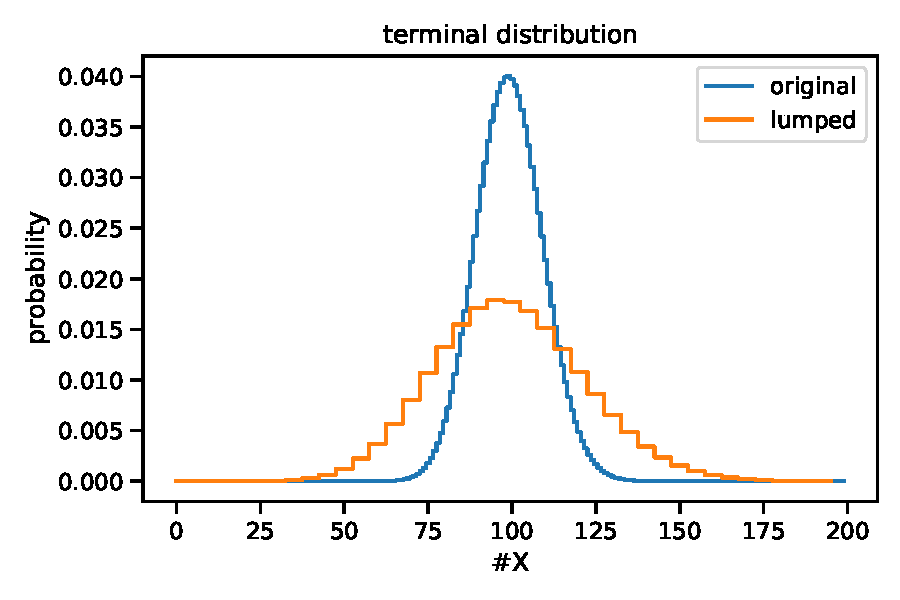
\includegraphics[scale=.3]{../gfx/lumped_dist.pdf}
            \end{figure}
        \end{column}
        \begin{column}{.6\textwidth}
            \begin{itemize}
                \item hyper-cube macro-states
                \item \emph{assumption}: uniform dist.\ within
                \item closed-form transition rates
            \end{itemize}
            \vspace{17mm}
            \begin{itemize}
                \item resulting distribution more ``flat''
                \item locate main probability mass
            \end{itemize}
            \vspace{4mm}
        \end{column}
    \end{columns}
\end{frame}

\begin{frame}{Stationary Distribution}{Finite-Space Projection}
    \begin{columns}
        \begin{column}{.32\textwidth}
            \begin{center}
                original\\
                \vspace{4mm}
                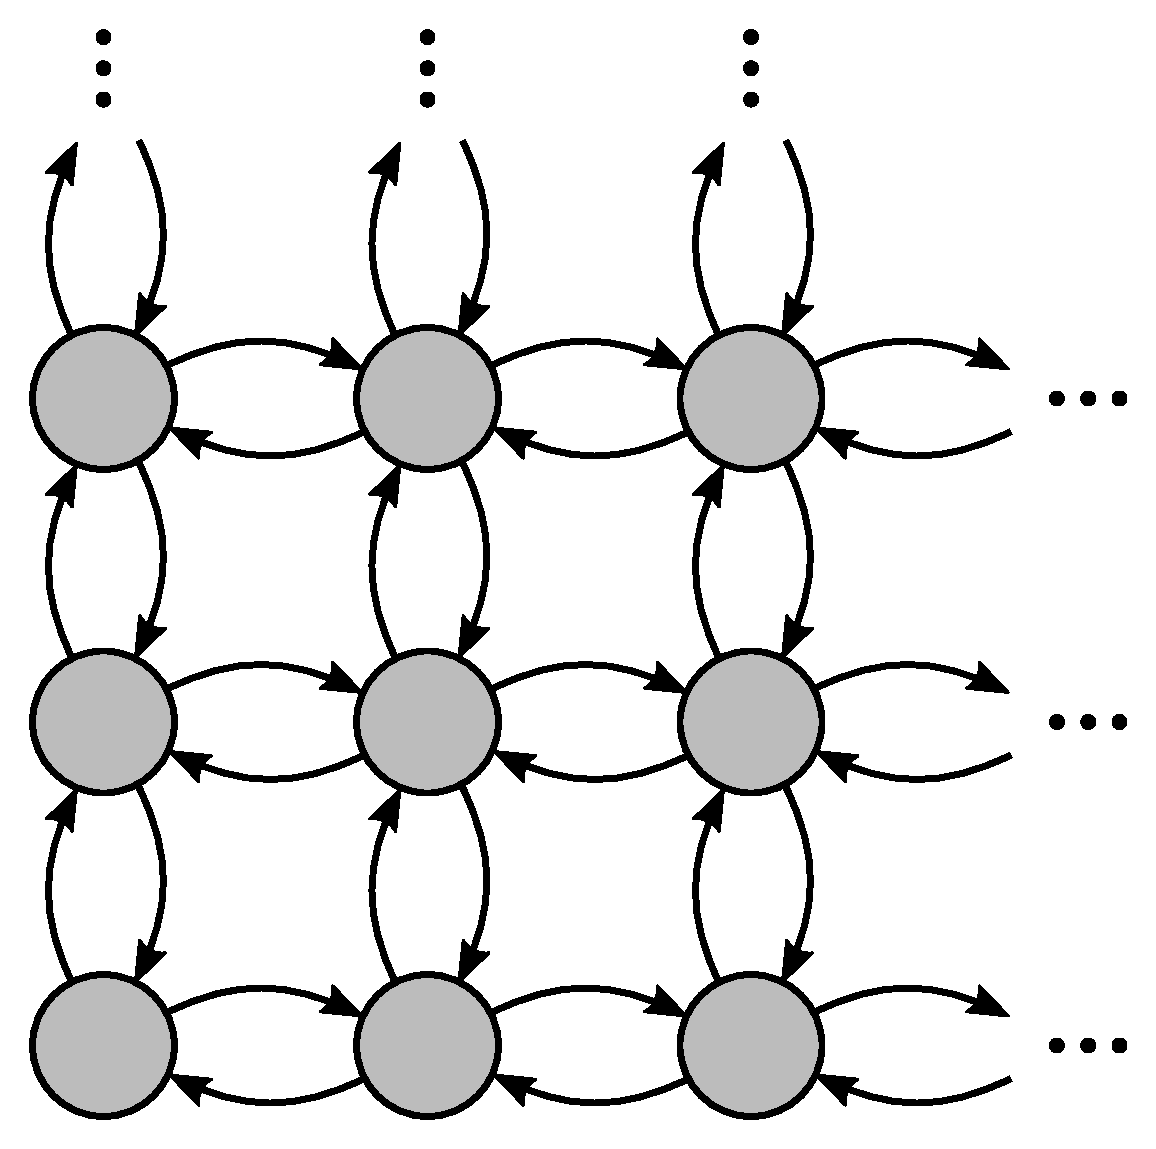
\includegraphics[height=2cm]{../gfx/state_space_untrunc.pdf}
            \end{center}
        \end{column}
        \begin{column}{.32\textwidth}
            \begin{center}
                sink state\\
                \vspace{4mm}
                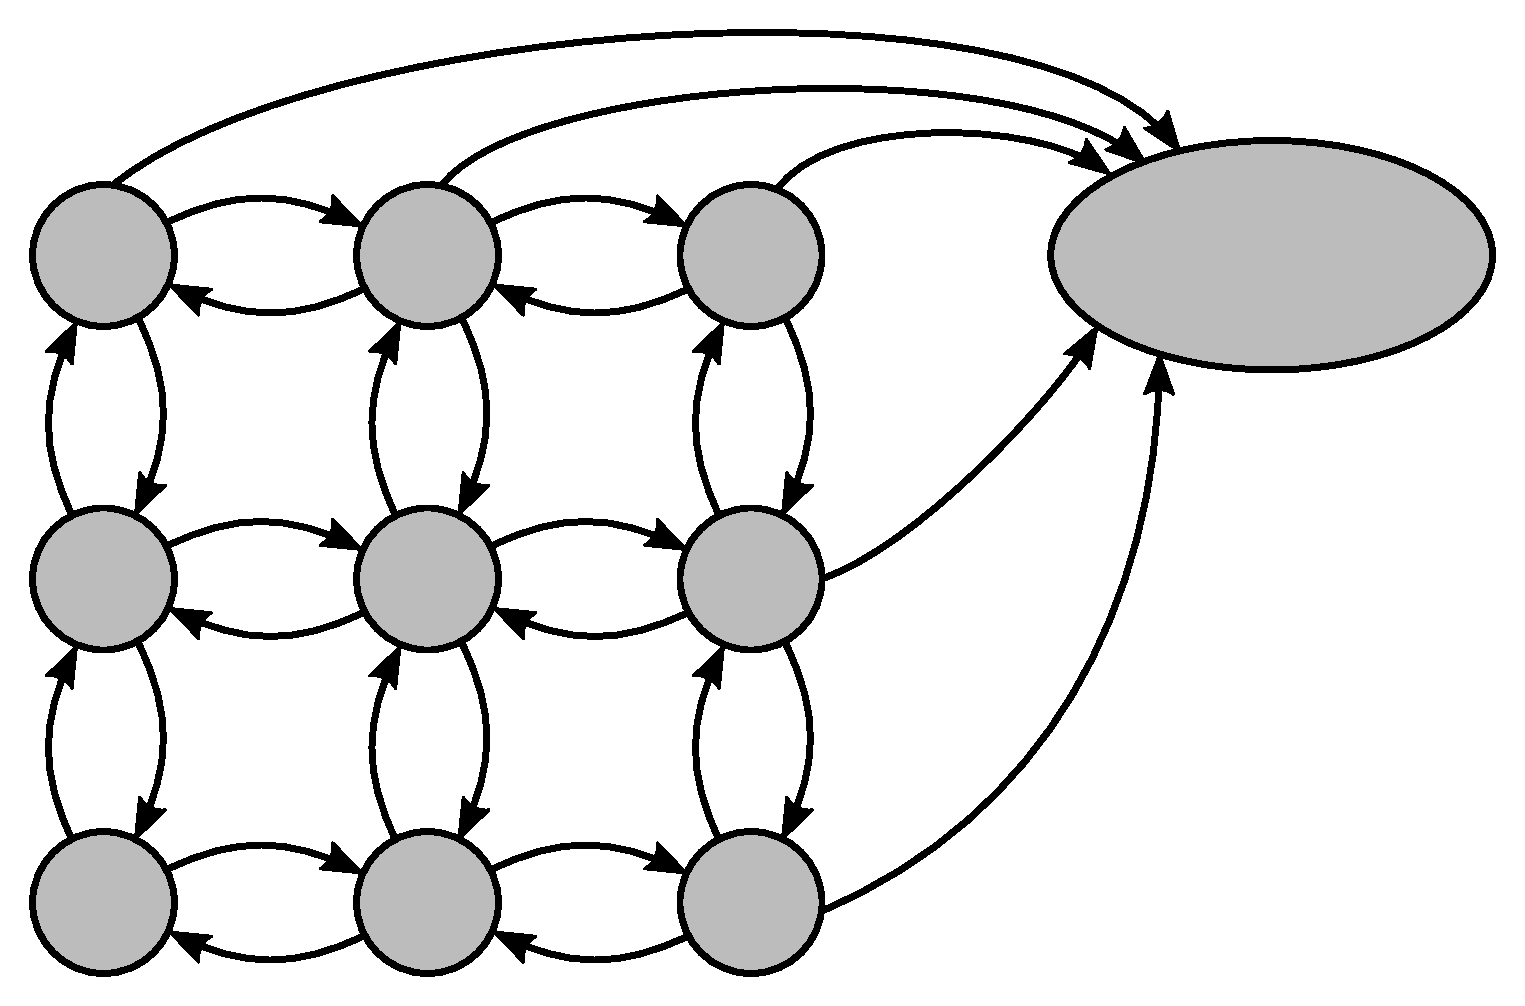
\includegraphics[height=2cm]{../gfx/state_space_redirected.pdf}
             \end{center}
        \end{column}
        \begin{column}{.32\textwidth}
            \begin{center}
                redirect\\
                \vspace{4mm}
                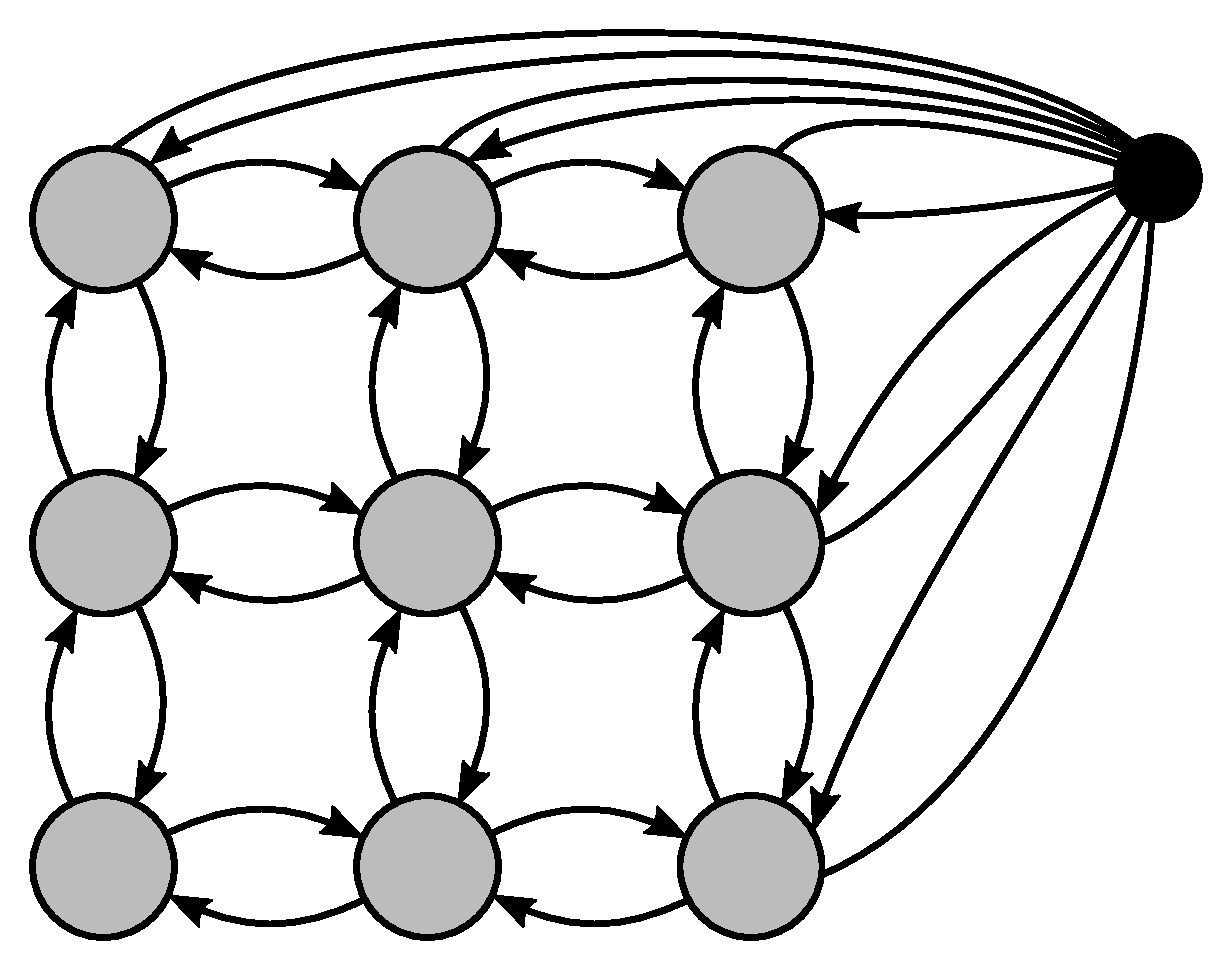
\includegraphics[height=2cm]{../gfx/state_space_reentry.pdf}
            \end{center}
        \end{column}
    \end{columns}
\end{frame}

\begin{frame}{Stationary Distribution}{Iterative Refinement Algorithm}
\end{frame}

\begin{frame}{Bridging Problem}{Dynamical Analysis Under Initial \emph{and} Terminal Constraints}
\end{frame}

\begin{frame}{Importance Sampling}
\end{frame}

\section{Conclusion}
\begin{frame}{Conclusions and Future Directions}
\end{frame}

\begin{frame}{Bibliography}
\end{frame}


\begin{frame}{Foster-Lyapunov Functions}
\end{frame}

\begin{frame}{Local Augmentation of Foster-Lyapunov Functions}
\end{frame}

\begin{frame}{Control Variates in General}
\end{frame}

\begin{frame}{Control Variates Selection Algorithm 1}
\end{frame}

\begin{frame}{Control Variates Selection Algorithm 2}
\end{frame}

\begin{frame}{Semi-definite programming}
\end{frame}

\end{document}
